\section{Overview of Text Retrieval Methods}

\subsection{How to Design a Ranking Function}
\begin{itemize}
\item \textbf{Query}: $q = q_1,\dots ,q_m$, where $q_i \in V$
\item \textbf{Document}: $d = d_1,\dots ,d_n$, where $d_i \in V$
\item \textbf{Ranking function}: $f(q,d) \in \Re$
\item \textbf{Key challenge}: how to measure the likelihood that document d is relevant to query q
\item \textbf{Retrieval model}: formalization of relevance (give a computational definition of relevance)
\end{itemize}


\subsection{Retrieval Models}
\begin{itemize}
\item \textbf{Similarity-based models}: $f(q,d) = similarity(q,d)$
    \begin{itemize}
    \item Vector space model
    \end{itemize}
\item \textbf{Probabilistic models}: $f(d,q) = p(R=1 \:\big|\: d,q)$, where $R \in {0,1}$ 
    \begin{itemize}       
    \item Classic probabilistic model
    \item Language model
    \item Divergence-from-randomness model    
    \end{itemize}
\item \textbf{Probabilistic inference model}: $f(q,d) = p(d \rightarrow q)$
\item \textbf{Axiomatic model}: $f(q,d)$ must satisfy a set of constraints
\end{itemize}    


\subsection{Common Ideas in State of the Art Retrieval Models}
\begin{figure}[H]
    \centering
    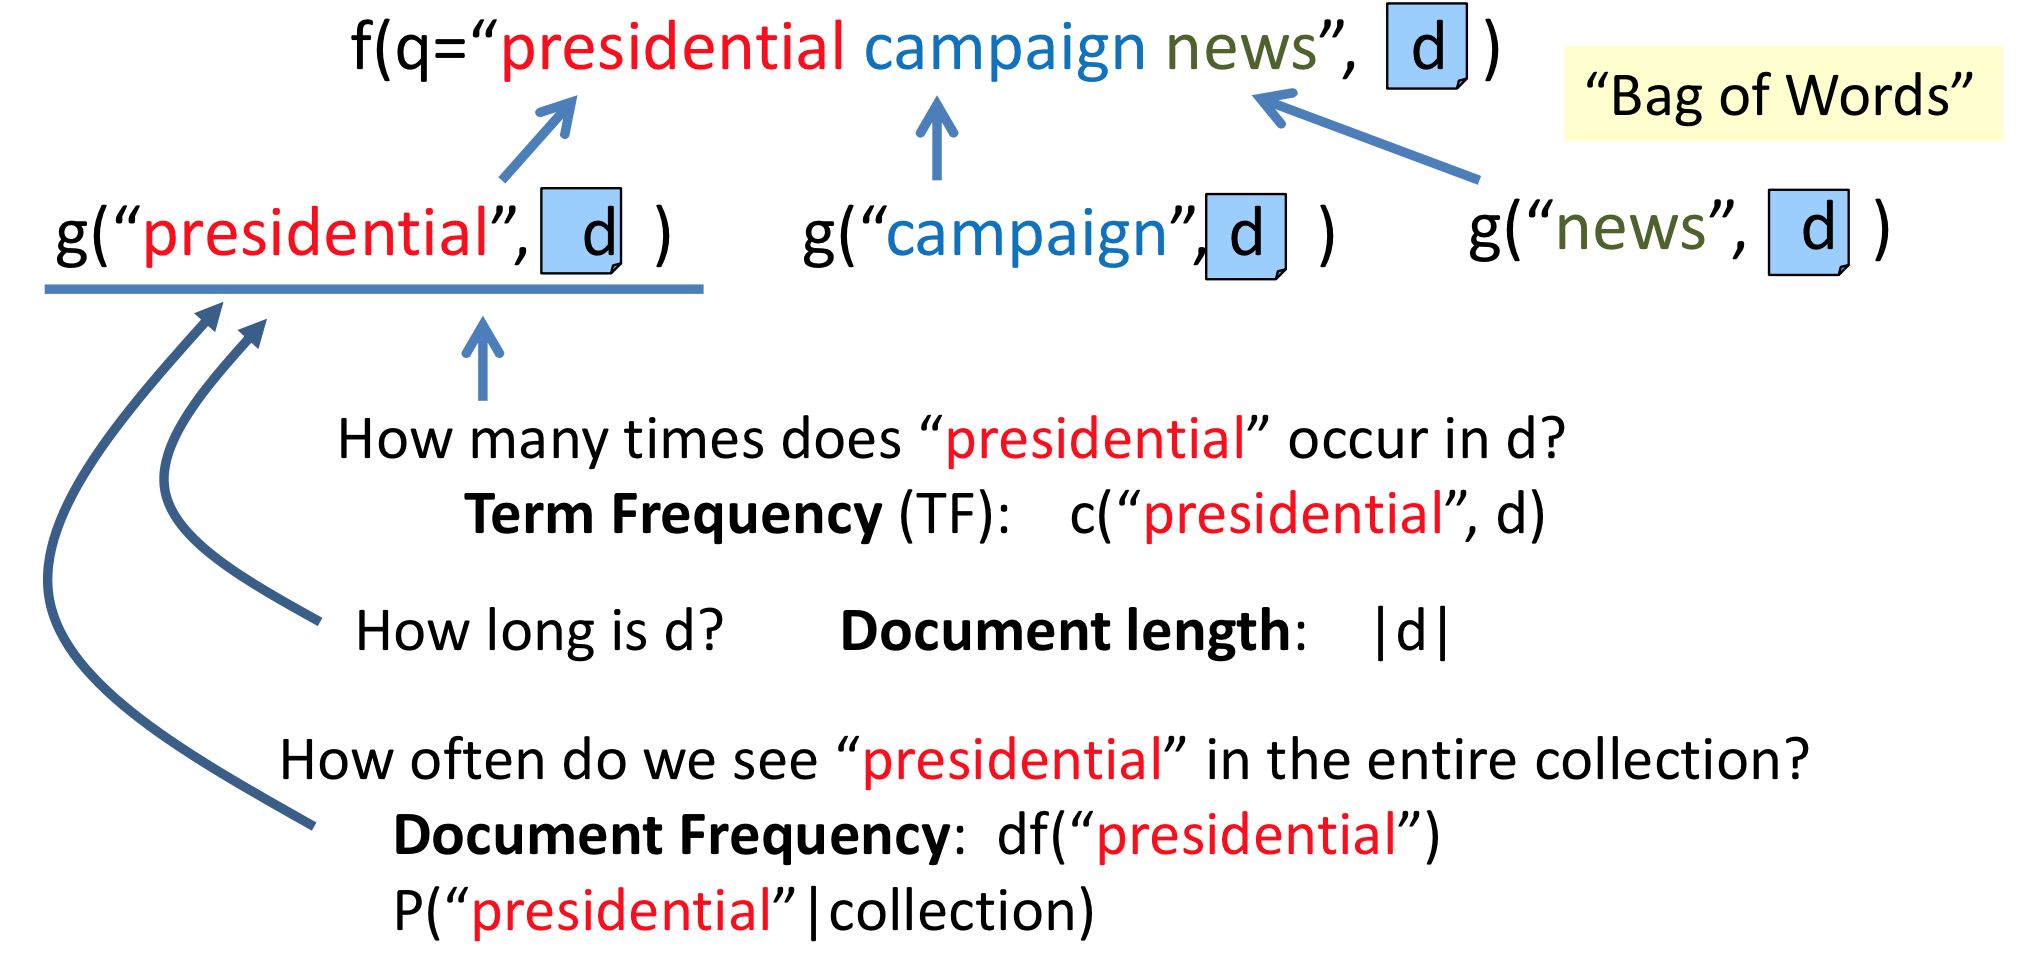
\includegraphics[width=\linewidth]{retrieval_models.png}
\end{figure}

State of the art ranking functions tend to rely on:
\begin{itemize}
\item Bag of words representation
\item Term Frequency (TF) and Document Frequency (DF) of words 
\item Document length
\end{itemize}

\subsection{Which Model Works the Best?}
When optimized, the following models tend to perform equally well [Fang et al. 11]:
\begin{itemize}
\item \textbf{Pivoted length normalization – BM25}
\item Query likelihood
\item PL2
\end{itemize}


\subsection{Recommended reading}
\begin{itemize}
\item Hui Fang, Tao Tao, and Chengxiang Zhai. 2011. <<Diagnostic Evaluation of Information Retrieval Models>>. ACM Trans. Inf. Syst. 29, 2, Article 7 (April 2011)
\item ChengXiang Zhai, <<Statistical Language Models for Information Retrieval>>, Morgan \& Claypool Publishers, 2008. (Chapter 2)
\end{itemize}
